%!TEX TS-program = xelatex
\documentclass[12pt, a4paper, oneside]{article}

\usepackage{amsmath,amsfonts,amssymb,amsthm,mathtools}  % пакеты для математики

\usepackage[english, russian]{babel} % выбор языка для документа
\usepackage[utf8]{inputenc} % задание utf8 кодировки исходного tex файла
\usepackage[X2,T2A]{fontenc}        % кодировка

\usepackage{fontspec}         % пакет для подгрузки шрифтов
\setmainfont{Linux Libertine O}   % задаёт основной шрифт документа

\usepackage{unicode-math}     % пакет для установки математического шрифта
\setmathfont[math-style=upright]{Neo Euler} % шрифт для математики

% Конкретный символ из конкретного шрифта
% \setmathfont[range=\int]{Neo Euler}

%%%%%%%%%% Работа с картинками %%%%%%%%%
\usepackage{graphicx}                  % Для вставки рисунков
\usepackage{graphics}
\graphicspath{{images/}{pictures/}}    % можно указать папки с картинками
\usepackage{wrapfig}                   % Обтекание рисунков и таблиц текстом

%%%%%%%%%%%%%%%%%%%%%%%% Графики и рисование %%%%%%%%%%%%%%%%%%%%%%%%%%%%%%%%%
\usepackage{tikz, pgfplots}  % язык для рисования графики из latex'a

%%%%%%%%%% Гиперссылки %%%%%%%%%%
\usepackage{xcolor}              % разные цвета

\usepackage{hyperref}
\hypersetup{
	unicode=true,           % позволяет использовать юникодные символы
	colorlinks=true,       	% true - цветные ссылки, false - ссылки в рамках
	urlcolor=blue,          % цвет ссылки на url
	linkcolor=red,          % внутренние ссылки
	citecolor=green,        % на библиографию
	pdfnewwindow=true,      % при щелчке в pdf на ссылку откроется новый pdf
	breaklinks              % если ссылка не умещается в одну строку, разбивать ли ее на две части?
}


\usepackage{todonotes} % для вставки в документ заметок о том, что осталось сделать
% \todo{Здесь надо коэффициенты исправить}
% \missingfigure{Здесь будет Последний день Помпеи}
% \listoftodos --- печатает все поставленные \todo'шки

\usepackage[paper=a4paper, top=20mm, bottom=15mm,left=20mm,right=15mm]{geometry}
\usepackage{indentfirst}       % установка отступа в первом абзаце главы

\usepackage{setspace}
\setstretch{1.15}  % Межстрочный интервал
\setlength{\parskip}{4mm}   % Расстояние между абзацами
% Разные длины в латехе https://en.wikibooks.org/wiki/LaTeX/Lengths


\usepackage{xcolor} % Enabling mixing colors and color's call by 'svgnames'

\definecolor{MyColor1}{rgb}{0.2,0.4,0.6} %mix personal color
\newcommand{\textb}{\color{Black} \usefont{OT1}{lmss}{m}{n}}
\newcommand{\blue}{\color{MyColor1} \usefont{OT1}{lmss}{m}{n}}
\newcommand{\blueb}{\color{MyColor1} \usefont{OT1}{lmss}{b}{n}}
\newcommand{\red}{\color{LightCoral} \usefont{OT1}{lmss}{m}{n}}
\newcommand{\green}{\color{Turquoise} \usefont{OT1}{lmss}{m}{n}}

\usepackage{titlesec}
\usepackage{sectsty}
%%%%%%%%%%%%%%%%%%%%%%%%
%set section/subsections HEADINGS font and color
\sectionfont{\color{MyColor1}}  % sets colour of sections
\subsectionfont{\color{MyColor1}}  % sets colour of sections

%set section enumerator to arabic number (see footnotes markings alternatives)
\renewcommand\thesection{\arabic{section}.} %define sections numbering
\renewcommand\thesubsection{\thesection\arabic{subsection}} %subsec.num.

%define new section style
\newcommand{\mysection}{
	\titleformat{\section} [runin] {\usefont{OT1}{lmss}{b}{n}\color{MyColor1}} 
	{\thesection} {3pt} {} } 


%	CAPTIONS
\usepackage{caption}
\usepackage{subcaption}
%%%%%%%%%%%%%%%%%%%%%%%%
\captionsetup[figure]{labelfont={color=Turquoise}}

\pagestyle{empty}

%%%%%%%%%% Свои команды %%%%%%%%%%
\usepackage{etoolbox}    % логические операторы для своих макросов

% Все свои команды лучше всего определять не по ходу текста, как это сделано в этом документе, а в преамбуле!

% Одно из применений - уничтожение какого-то куска текста!
\newbool{answers}
\booltrue{answers}
%\boolfalse{answers}

\usepackage{enumitem}
% бульпоинты в списках
\definecolor{myblue}{rgb}{0, 0.45, 0.70}
\newcommand*{\MyPoint}{\tikz \draw [baseline, fill=myblue,draw=blue] circle (2.5pt);}
\renewcommand{\labelitemi}{\MyPoint}

% расстояние в списках
\setlist[itemize]{parsep=0.4em,itemsep=0em,topsep=0ex}
\setlist[enumerate]{parsep=0.4em,itemsep=0em,topsep=0ex}


\begin{document}
	
\section*{Семинар 4: Градиентный спуск}

\subsection*{Задача 0 (задача с семинара из прошлого семестра)}

Давайте попробуем совсем-совсем на пальцах почувствовать как модели обучаются. Пусть у Хозяина мемов есть две переменные: $x$ --- возраст подписчика, $y$ --- число лайков, которое он оставил. Хозяин мемов хочет оценить регрессию $y = \beta \cdot x$, то есть он хочет попытаться предсказать число лайков по возрасту подписчика. Хозяин собрал два наблюдения для оценивания модели: $x_1 = 15, y_1 = 10$ и $x_2 = 22, y_2 = 2$.

Теперь хозяину надо подобрать коэффициент $\beta$ так, чтобы ошибка прогноза, измеряемая с помощью $MSE$ оказалась поменьше. 

\begin{enumerate} 
	\item  Пусть $\beta = 1$. Какие значения нам спрогнозирует модель? Какая у неё будет ошибка? 
	
	\item Пусть $\beta = 0.5$. Найдите прогнозы и ошибку модели. 
	
	\item  Какое значение для $\beta$ нам больше подходит? Как можно найти оптимальное $\beta$? 
\end{enumerate}  

\ifbool{answers}{
	\textbf{Решение:}
	
	При $\beta = 1$ получаем прогнозы $\hat y_1 = 1 \cdot 15 = 15  \hat y_2 = 1 \cdot 22 = 22$. Находим ошибку: $MSE = (15 - 10)^2 + (22 - 2)^2 = 25 + 400 = 425$. 
	
	При $\beta = 0.5$ получаем прогнозы $\hat y_1 = 5$ и $\hat y_2 = 7.5$. Ошибка составит $MSE = (10 - 5)^2 + (7.5 -2)^2 = 25 + 30.25 = 55.25$. 
	
	В случае $\beta = 0.5$ ошибка ниже. Методом перебора мы можем найти оптимальное значение $\beta$ для нашей формулы. Конечно же на практике компьютеры не перебирают влоб все возможные значения. Они делают перебор по-умному. Обычно находят производную функции ошибки по параметру $\beta$ и по ней понимают куда надо шагать и какое значение $\beta$ надо проверить на "оптимальность" следующим. Такой перебор называется градиентным спуском.  Но о нём мы поговорим подробнее как-нибудь в другой раз.  {\color{red}  \textbf{ЭТОТ ДЕНЬ НАСТАЛ!} }
}


\subsection*{Задача 1}

Маша услышала про машин лёрнинг и решила, что они и есть та самая Маша, которой этот лёрнинг принадлежит.  Маша измерила вес трёх упаковок с конфетками,  $y_1=6$, $y_2=6$, $y_3=10$.  Она хочет спрогнозировать вес следующего пакетика. Модель для веса пакетиков у Маши очень простая,  $y_i = \beta + u_i, $ поэтому прогнозирует Маша по формуле $\hat y_i = \hat \beta$.

Для оценки параметра $\beta$ Маша использует следующую целевую функцию:

\[
L = MSE = \sum (y_i - \hat \beta)^2 
\]


\begin{enumerate}
	\item[a)] Найдите оптимальное $\hat \beta$. Для этого найдите минимум $MSE$. 
	\item[б)] Сделайте три шага стохастического градиентного спуска.  Пусть в алгоритм попадает сначала первое наблюдение, потом второе, потом третье. В качестве стартовой точки используйте $\beta_0= 0$ .В качестве скорости обучения возьмите $\gamma = 0.1.$
\end{enumerate}

\ifbool{answers}{
	\textbf{Решение:}
	
\begin{enumerate}
	\item[a)]  В пункте а Маша хочет подобрать модель, которая будет прогнозировать вес нового пакетика с конфетками. Для этого она руководствуется принципом минимизации квадрата ошибки. Если бы Маша спрогнозировала, что первый пакетик будет весить $\beta$, она бы ошиблась на $(6 -  \beta)^2$. Если бы Маша спрогнозировала, что второй пакетик будет весить $\beta$, она бы ошиблась на $(6 - \beta)^2$.  В случае третьего пакетика ошибка составила бы $(10 -  \beta)^2$.  Наша дальнейшая задача --- минимизируя суммарную ошибку Маши, получить хорошую оценку для $\beta$: 
		
	\[L(\beta) = (6 - \beta)^2 + (6 -  \beta)^2 + (10 -  \beta)^2 \to \min_{ \beta}.\]
	
	Давайте вспоминать 11 класс школы. ОХ! Как же давно это было. Как найти экстремум функции? Взять производную и приравнять её к нулю! 
	
	\[  -4 \cdot (6 - \beta) - 2 \cdot (10 - \beta) = 0 \Rightarrow \hat \beta = \frac{44}{6} \approx 7.3. \]
	
	Итак, если Маша хочет строить для каждого последущего пакетика прогнозы с помощью одного числа, и при этом она минимизирует квадратичную ошибку, наименьшие потери даст прогноз $7.3$. Если конечно верить данным. 
	
	Если нарисовать $L(\beta)$ на картинке, то можно увидеть, что минимум ошибки, действительно, достигается в точке $7.3$.
	
	\begin{center}
		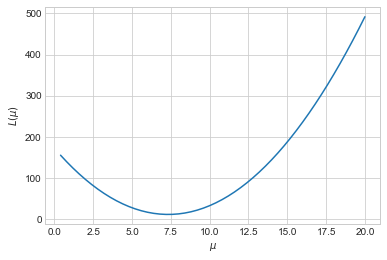
\includegraphics[scale=0.45]{mul.png}
	\end{center}
	
	На паре мы сказали, что для трёх наблюдений и нам и компьютеру решить такое уравнение довольно просто, но когда наблюдений много тысяч, решать придётся долго. Хочется получать то же самое решение, но на порядок быстрее. Для этого придумали градиентный спуск.
	
	
	\item[б)]  Займёмся градиентным спуском. Стартовать будем из точки $\beta_0 = 0$. Нам хочется пометь нашу $\beta$ так, чтобы оказаться ближе к оптимальной точке. В нулевое задачке мы выбрали два рандомных значения $\beta$ и посмотрели какое из них лучше. Можно было бы поступить аналогично: выбрать много разных цифр и посмотреть где $MSE$ будет самым маленьким. Но это тоже долго.	Хочется перебирать $\beta$ как-то по умному. 
	
	Что такое производная? Производная --- это просто, скорость роста, это просто --- скорость роста.  То есть если мы стоим около подножия горы, и мы знаем какая именно функция описывает выпуклости этой горы, и нам хочется на эту гору залезть, если мы найдём производную, она покажет как быстрее всего можно это сделать. 
	
	В случае нашей задачки мы стоим в точке $\beta_0 = 0$. Нам хочется побыстрее сползти в точку минимума $MSE$.  Значит нужно идти против $MSE'_{\beta}$.  Давайте сделаем это. 
	
	По условию задачи в наши цепкие руки сначала попадает $y = 6$. Найдём производную 
	
	$$
	MSE'_{\beta} = ((6 - \beta)^2 )'_{\beta}= -2 \cdot (6 - \beta) 
	$$

	Получается, что из $\beta = 0$ надо шагать на $(-1) \cdot -2 \cdot (6 - 0) = 12$. Обычно никто не шагает на всю величину, чтобы случайно не пробежать мимо оптимальной точки. Шаги умножают на специальный коэффициент $\gamma$, скорость шагания (или скорость обучения). У нас это $0.1$. Наконец, делаем шаг: 
	
	$$
	\beta_1 = \beta_0 - 0.1 \cdot MSE'(\beta_0) = 0 + 0.1 \cdot 12 =  1.2
	$$
	
	Если мы всё селали правильно, наша ошибка $MSE$ должна была стать меньше. Проверим это. Когда мы были в нуле, мы ошибались на $MSE(0) = (6 - 0)^2 = 36$.  Теперь мы ошибаемся на $MSE(1.2) = (6 - 1.2)^2 = 23.04$. Ура! Стало лучше.  
	
	Обратите внимание, что нельзя взять $\beta = 6$. Для первого наблюдения, мы и правда получим $MSE=0$, но когда в наши цепкие руки попадёт $y=10$ мы крупно ошибемся. Мы хотим уменьшить ошибку для всей выборки, а не для одного конкретного наблюдения. 
	
	Второй шаг. У нас в руках снова $y = 6$: 
	
	$$
	\beta_2 = \beta_1 - 0.1 \cdot (-2) \cdot (6 - \beta_1) = 1.2 + 0.96 = 2.16
	$$
	
	Ну и последний шаг. У  нас в руках $y = 10$. 
	
	$$
	\beta_3 = \beta_2 - 0.1 \cdot (-2) \cdot (10 - \beta_2) = 2.16 + 0.1 \cdot 15.68 = 3.73
	$$
	
	С каждом шагом мы всё ближе к оптимальной точке $7.3$.  Но вот незадача! Наблюдения закончились. Что делать?  Пойти по второму кругу! Так обычно делают на практике. Один проход по всем данным даже называют пафосным словом "эпоха". 
	
	Более того, на практике обычно берут наблюдения для обучения (поиска производных) не по порядку, а в случайном порядке. Такую модификацию градиентного спуска называют стохастическим градиентным спуском. 
	
	Другой вопрос: а когда успокаиваться и останавливать алгоритм? Обычно останавливаются, когда два соседних $\beta_t$ отличаются друг от друга на какую-то совсем маленькую величину:
	
	$$
	|\beta_{t+1}  - \beta_t|  < 0.00000000001.
	$$
	
	Тогда говорят, что алгоритм сошёлся. Когда в питоне вы пишите \textbf{model.fit(Xtr, ytr)}, линейные модели обучаются именно с помощью градиентного спуска. 
\end{enumerate}
}


\subsection*{Задача 2}

Маша, у которой есть лёрнинг,  услышала про переобучение. В умной книге она вычитала, что признаком переобучения в линейных моделях являются очень большие коэффициенты. Чтобы побороть переобучение, можно попытаться штрафовать коэффициенты за их размеры. Есть целых две модели, которые позволяют это сделать:  Ridge-регрессия и Lasso-регрессия. Маша решила использовать Ridge для  её для задачки с конфетами.  

Маша измерила вес трёх упаковок с конфетками,  $y_1=6$, $y_2=6$, $y_3=10$.  Она хочет спрогнозировать вес следующего пакетика. Модель для веса пакетиков у Маши очень простая,  $y_i = \beta + u_i, $ поэтому прогнозирует Маша по формуле $\hat y_i = \hat \beta$.

Для оценки параметра $\beta$ Маша использует новую целевую функцию:

\[
L = \sum (y_i - \hat \beta)^2  + \alpha \cdot \beta^2
\]

Именно такую функцию использует Ridge-регрессия. Слагаемое $\alpha \cdot \beta^2$ это и есть штраф за слишком большие коэффициенты.  Множитель $\alpha$ --- это сила штрафа. Когда вы делали домашку, вы пытались в своих моделях указывать его. 


\begin{enumerate}
	\item[a)] Найдите оптимальное $\hat \beta$. Для этого найдите минимум $L$. 
	\item[б)] Пусть маша решила, что $\alpha = 2$.  Сделайте три шага стохастического градиентного спуска.  Пусть в алгоритм попадает сначала первое наблюдение, потом второе, потом третье. В качестве стартовой точки используйте $\beta_0= 0$ .В качестве скорости обучения возьмите $\gamma = 0.1.$
\end{enumerate}

\ifbool{answers}{
	\textbf{Решение:}
	
	\begin{enumerate}
			
\item[а)]  Усложняем задачу. Теперь мы обучаем модель, но уже  с гиперпараметром $\alpha$. Правда непонятно нафига нам этот гиперпараметр сдался. Давайте попробуем точно также, как в предыдущей задачке, минимизировать ошибку с участием гиперпараметра и посмотреть на то как наши прогнозы $\beta$ зависят от него. 
	
\[L(\beta) = (6 - \beta)^2 + (6 -  \beta)^2 + (10 -  \beta)^2 + \alpha \beta^2 \to \min_{ \beta}.\]
		
Снова берём производную. Всё, как в школе учили. 
	
\begin{equation*}
\begin{aligned}
	&-4 \cdot (6 - \beta) - 2 \cdot (10 - \beta) + 2\beta \alpha = 0  \\
	&44 = 6 \beta + 2 \alpha \beta \\
	&22 = 3 \beta + \alpha \beta \\
	&22 = \beta(3 + \alpha) \\
	&\hat \beta = \frac{22}{3 + \alpha}
\end{aligned}
\end{equation*}
	
Отлично. Теперь у нас есть зависимость наших прогнозов от гиперпараметра в явном виде. Давайте попробуем посмотреть как выглядит эта зависимость на графике. 	

\begin{center}
	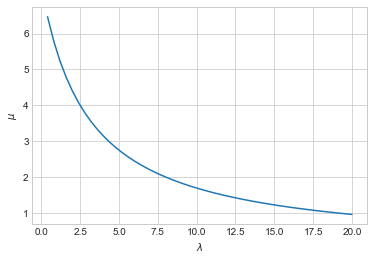
\includegraphics[scale=0.45]{lambda_mu.png}
\end{center}

Гиперпараметр альфа обладает интересным эффектом. Он зануляет значение $\beta$, если оказывается очень большим.  Именно так работает регуляризация. Она стягивает коэффициенты к нулю. Когда модель слишком сильно подстраивается под данные, коэффициенты в ней оказываются очень большими. 

\begin{center}
	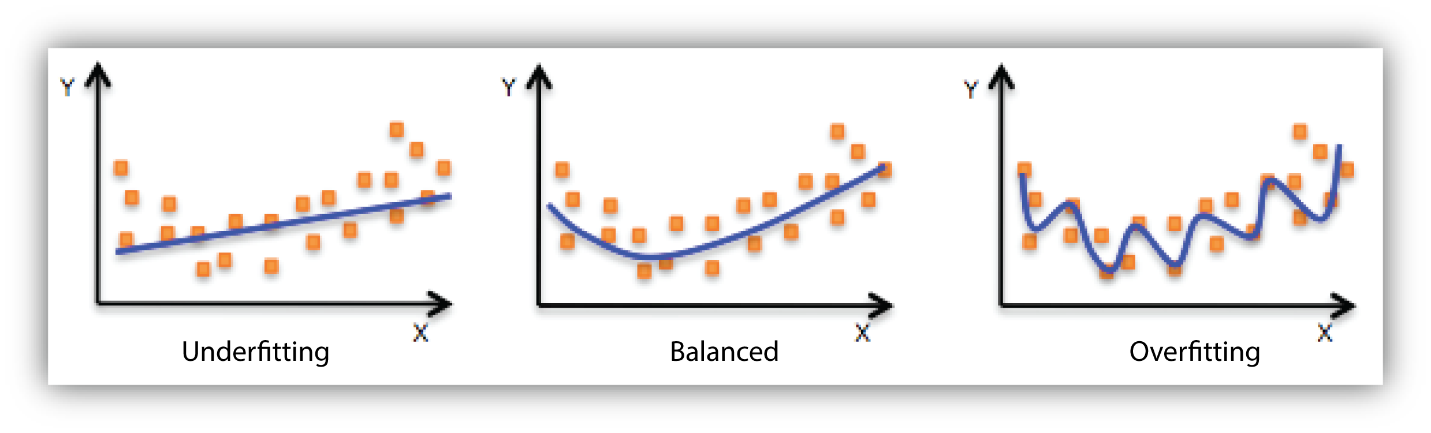
\includegraphics[scale=1]{overfit.png}
\end{center}

Стягивание к нулю запрещает модели слишком сильно подстраиваться под данные. 

Получается, что меняя гиперпараметр $\alpha$, мы можем давать бой переобучению модели и, варьируя его, улучшать прогнозную силу. Возникает вопрос: а как выбрать оптимальное значения для $\alpha$? Давайте вспомним предыдущий семинар и то, как мы делали это с муравьями, когда подбирали оптимальное число соседей для нашего алгоритма. 
		
Мы закрывали одного муравья ладошкой, на оставшихся обучали классификатор, а затем смотрели куда будет относиться закрытый ладошкой муравей. Сделав так с каждым муравьём, мы смотрели сколько ошибок допустили при $k=3$ и при $k=4$, и брали такое $k$, для которого ошибок было меньше. Говоря иначе, мы с помощью кросс-валидации <<выкинь одного>> по решётке подобрали оптимальное значение для гиперпараметра $k$, которое позволило нам получить хорошие прогнозы.

Здесь можно поступить аналогичным образом.  Именно этим занимался в вашей домашке \textbf{Gridsearch.}
		
\item[б)]  Теперь сделаем на тех же данных пару шагов градиентного спуска.  Стартуем из $\beta = 0$, идём со скростью $\gamma = 0.1$.  По условию задачи $\alpha = 1$. Поехали: 

$$
L'_{\beta} =  -2 \cdot (y_i - \beta) + 2 \cdot \alpha \cdot \beta 
$$

Делаем первый шаг: 

$$
\beta_1 = \beta_0 -  \gamma \cdot [ (-2) \cdot  (y_i - \beta_0) + 2 \cdot \alpha \cdot \beta_0] = 0 + 0.1 \cdot [12 - 4 \cdot 0] = 1.2
$$

Второй шаг: 

$$
\beta_2 = \beta_1 -  \gamma \cdot [ (-2) \cdot  (y_i - \beta_1) + 2 \cdot \alpha \cdot \beta_1] = 1.2 + 0.48 = 1.68
$$

Третий шаг: 

$$
\beta_3 = 1.68 - 0.1 \cdot (-2 \cdot (10 - 1.68) + 2 \cdot 2 \cdot 1.68) ) = 4.016
$$

	\end{enumerate}
}



\subsection*{Задача 3}

	Маша Нестерова, хозяйка машин лёрнинга,  собрала два наблюдения: $x_1 = 1, x_2 = 2$, $y_1 = 2, y_2 = 3$ и собирается обучить линейную регрессию $y = \beta \cdot x$.  Маши очень хрупкая девушка, и ей не помешает помощь. 

\begin{enumerate}
\item[а)] Получите оценку методом наименьших квадратов (минимизируя $MSE$ и беря производную).
	
\item[б)]   Сделайте два шага стохастического градиентного спуска. В качестве стартовой точки используйте $\beta_0 = 0$.  В качестве скорости обучения возьмите $\eta = 0.1$.  Пусть в градиентный спуск сначала попадает первое наблюдение, затем второе. 

\item[в)]   Возможно, что имеет смысл попробовать решить эту же задачку для случая, когда к MSE добавляется $\alpha \cdot \beta^2$ (Ridge регрессия). Возможно, Филипп именно её приготовил для самостоятельной.  В качетсве $\alpha$ возьмите $3$. 
\end{enumerate}

\ifbool{answers}{
	\textbf{Решение:}

\begin{enumerate}
\item[а)]  Пример решения есть в "ещё задачах". 

\item[б)]  Я верю в тебя, поднажми :) 

\item[в)]  Именно та задача, которую ты не решил, тебе и попадётся.
	
\end{enumerate}	
}



\section*{Ещё задачи}

Задачки из этого раздела можно не решать, но они открывают чакры. Если хотите шарить, посмотрите их. 

\subsection*{Задача 4}

Маркетологи Вова и Вася строили регрессию $y = \beta_0 + \beta_1 x$. Каждый оценивал её по своим данным. У Васи получилось, что $\hat \beta_1 = 2$, у Вовы получилось, что $\hat \beta_1 = 8$.

Пришла Алиса, отобрала у Вовы и Васи данные, соединила их вместе и построила регрессию сразу на всём. У неё получилось, что $\hat \beta_1 = -10$. Может ли такое быть?

\ifbool{answers}{
	\textbf{Решение:}
	
Конечно может быть! Надо лишь немного пофантазировать.  Пусть выборки Васи и Вовы имеют следущий вид: 

\begin{center}
	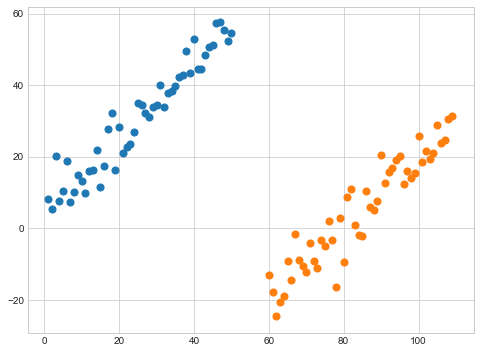
\includegraphics[scale=0.5]{VVA_1.png}
\end{center}

Если они попробуют построить свои линии регрессии, они получат положительные коэффициенты наклона. При этом, если неожиданно придёт Алиса и отберёт у них выборки, она получит отрицательный наклон у своей прямой.

\begin{center}
	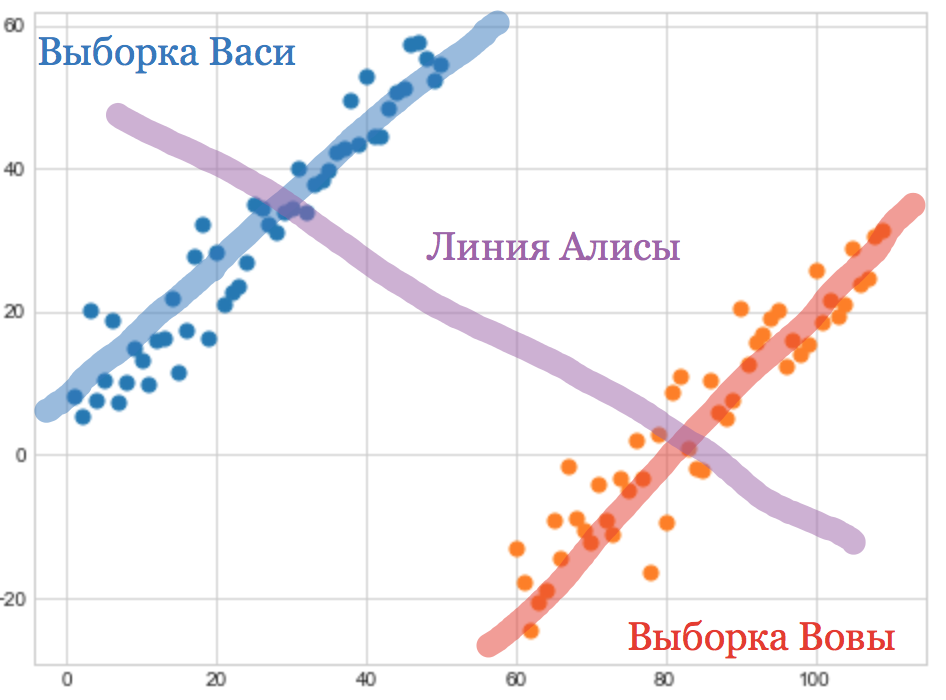
\includegraphics[scale=0.25]{VVA_2.png}
\end{center}
	
}

\subsection*{Задача 5}

Каждый день Маша ест конфеты и решает задачи по машинному обучению. Пусть $x_i$ — количество решённых задач, а $y_i$ — количество съеденных конфет.

\begin{center}
\begin{tabular}{c|c}
	\hline
	$x_i$ & $y_i$ \\
	\hline
	1 & 1 \\
	2 & 2 \\
	2 & 8 \\
\end{tabular}
\end{center}

Рассмотрим модель $y_i = \beta x_i + u_i$. Маша использует функцию потерь 
\[
\sum (y_i - \hat \beta x_i )^2
\]

\begin{enumerate}
	\item[а)] Найдите МНК-оценку $\hat \beta$ для имеющихся трёх наблюдений.
	\item[б)] Нарисуйте исходные точки и полученную прямую
	регрессии.
	\item[в)] Выведите формулу для $\hat \beta$ в общем виде для $n$ наблюдений.
	\item[г)] На семинаре по машинному обучению неожиданно выяснилось, что Миша тоже каждый день решает задачи по машинному обучению. Правда он более сдержан в плане конфет. Миша решил взять Машины наблюдения и с помощью функционала 
	\[
	\sum |y_i - \hat \beta x_i |
	\]  
	
	оценить $\beta$. Помогите Мише найти оценку. 
	\item[д)] К поеданию конфет решает присоединиться Вадик. У него тоже есть своя функция потерь
	\[
	\sum (y_i - \hat \beta x_i)^2 + 3\beta^2
	\]  	
	Оцените $\beta$ для его случая. Нарисуйте все три прямые на одной картинке и порассуждайте почему они получились именно такими, какими получились. 
\end{enumerate}

\ifbool{answers}{
	\textbf{Решение:}
	
\begin{enumerate}
	\item[а)] Текущая модель немного посложнее модели из третьей задачи. Тем не менее, она решается ровно по такой же схеме. Выписываем ошибку и минимизируем её по параметрам модели: 
	
	\[ (1- \beta)^2 + (2 - 2 \beta)^2 + (8 - 2 \beta)^2 \to \min_{\beta} \]
	
	Берём производную и приравниваем её к нулю: 
		
	\begin{equation*}
	\begin{aligned}
	& -2(1-\beta) - 4(2-2\beta) - 4(8-2\beta) = 0, \\
	& (1-\beta) + 2(2 - 2 \beta) + 2(8 - 2 \beta) = 0, \\
	&  9 \beta = 21, \\
	&  \hat \beta = \frac{21}{9}.\\
	\end{aligned}
	\end{equation*}	
	
	Итоговая модель для строительства прогнозов: $y = \frac{21}{9} \cdot x$. Обратите внимание, что в данном случае мы оценивали именно зависимость $y$ от $x$. Для каждого $x$ будет свой прогноз $y$. 
	
	\item[б)]  Написуем наши наблюдения и оценённую прямую на одной картиночке! 
	
	\begin{center}
		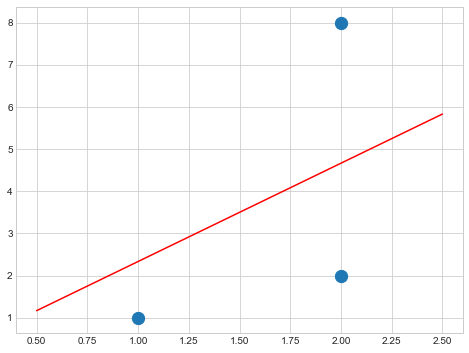
\includegraphics[scale=0.5]{reg_81.png}
	\end{center}
	
	
	\item[в)]  Выведем формулу для случая $n$ наблюдений. Ошибка будет иметь вид: 
	
	\[(y_1 - \beta x_1)^2 + (y_2 - \beta x_2)^2 + \ldots + (y_n - \beta x_n )^2 \to \min_{\beta} \]
	
	Берём производную! 
	
	\begin{equation*}
	\begin{aligned}
	&  -2 x_1 (y_1 - \beta x_1) - 2 x_2 (y_2 - \beta x_2) - \ldots -2 x_n (y_n - \beta x_n) = 0 \\
	& x_1 (y_1 - \beta x_1) +  x_2 (y_2 - \beta x_2) + \ldots +  x_n (y_n - \beta x_n) = 0  \\
	& x_1 y_1 - \beta x_1^2 + x_2 y_2 - \beta x_2^2 + \ldots + x_n y_n - \beta x_n^2 = 0\\
	& x_1 y_1 + \ldots + x_n y_n = \beta (x_1^2 + \ldots + x_n^2) \\
	\end{aligned}
	\end{equation*}
	
	В итоге получаем, что $\hat \beta = \frac{x_1 y_1 + \ldots + x_n y_n}{x_1^2 + \ldots + x_n^2}$ или, более лаконично записывая, $\hat \beta = \frac{\sum_{i=1}^{n} x_i y_i }{\sum_{i=1}^n x_i^2}.$
	
	\item[г)] Выписываем ошибку Миши
	
	\[ |1- \beta| + |2 - 2 \beta| + |8 - 2 \beta|  \to \min_{\beta}. \]
	
	У нас проблемы. От модуля нельзя взять производную. К счастью, у нас мало наблюдений и и мы можем нарисовать нашу функцию потерь. Она будет кусочно-линейной. У неё будет две особые точки: $1$ и $8$.  Посмотрим как ведёт себя наша функция до точки $1$. Раскрываем модули и получаем поведение функции на промежутке от минус бесконечности до $1$: 
	
	\[ 1 - \beta + 2 - 2\beta + 8 - 2\beta = 11 - 5\beta.\] 	
	
	Теперь раскрываем модули на отрезке от $1$ до $4$: 
	
	\[ - 1 + \beta - 2 + 2\beta + 8 - 2\beta = 5 + \beta.\] 
	
	Раскрываем модули на промежутке от $4$ до конца: 
	
	\[ - 1 + \beta - 2 + 2\beta  - 8 + 2\beta = -11 + 5 \beta. \]
	
	Изобразим нашу функцию потерь на картинке. 
	
	\begin{center}
		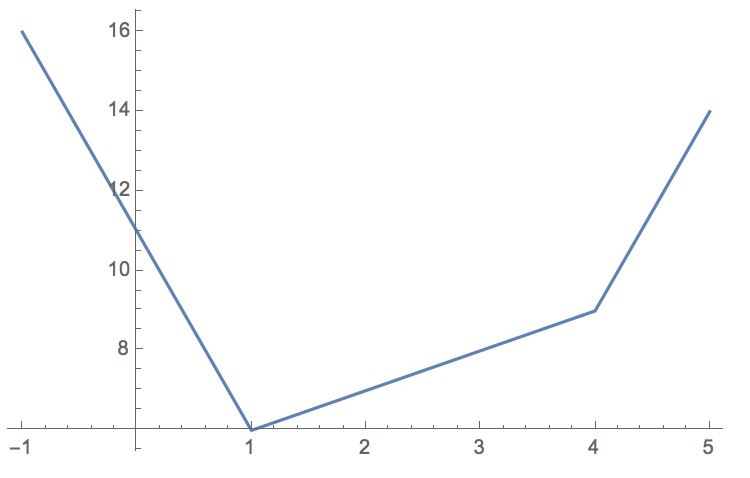
\includegraphics[scale=0.4]{reg_82.png}
	\end{center}
	
	Функция достигает минимума в точке $1$, получается что $\hat \beta = 1$. 
	
	\item[д)]  У Вадика модель с регуляризатором. Не факт, что $\lambda$ в его случае выбрана оптимально. При желании можно попробовать подобрать оптимальное значение, используя ту же стратегию, что и в третьей задаче. Минимизируем ошибку Вадика. 
	
		\[ (1- \beta)^2 + (2 - 2 \beta)^2 + (8 - 2 \beta)^2 + 3 \beta^2 \to \min_{\beta} \]
		
	Берём производную: 
	
		\begin{equation*}
	\begin{aligned}
	& -2(1-\beta) - 4(2-2\beta) - 4(8-2\beta) + 6 \beta = 0, \\
	& (1-\beta) + 2(2 - 2 \beta) + 2(8 - 2 \beta) - 3\beta = 0, \\
	&  12 \beta = 21, \\
	&  \hat \beta = \frac{21}{12}.\\
	\end{aligned}
	\end{equation*}	
	
	Видим, что из-за наличия регуляризатора, коэффициент $\beta$ уменьшился.  Нарисуем все три линии регрессии на одной картинке и немного порассуждаем о них. 
	
	\begin{center}
		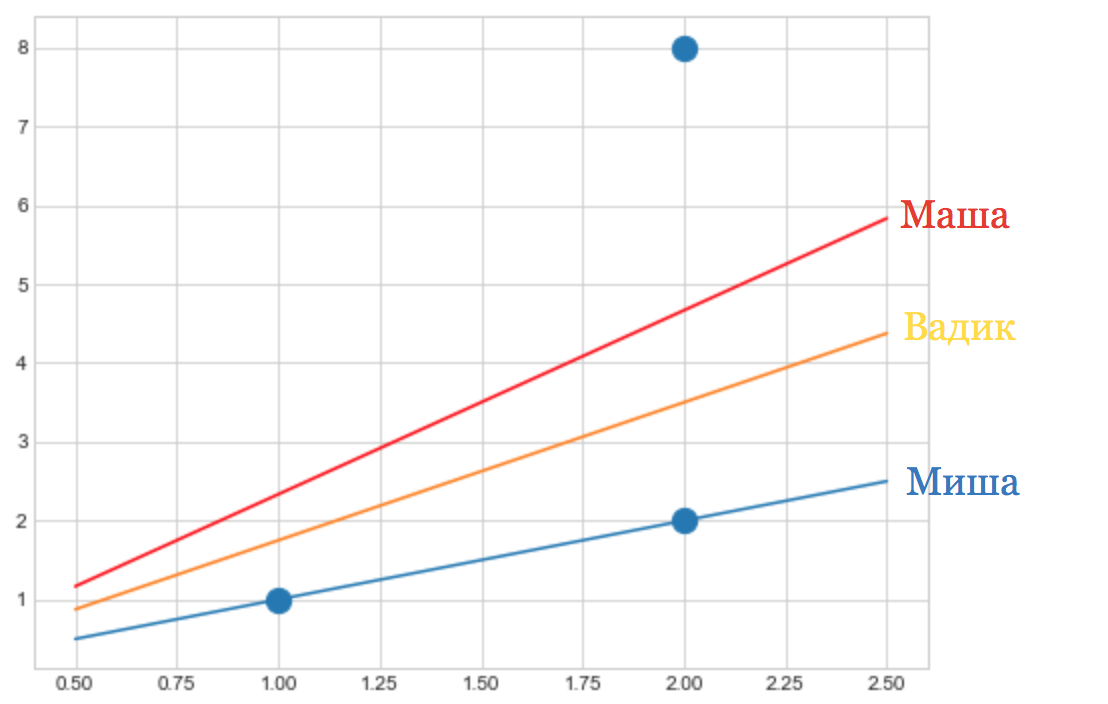
\includegraphics[scale=0.3]{reg_83.png}
	\end{center}
	
	Точка $(2,8)$ сильно выделяется. Это выброс. Машина линия довольно сильно под этот выброс подстраивается. Модель переобучается под выборку. Модель Вадика более устойчива. Из-за регуляризатора она оказывается ниже Машиной.
	
	Модель Миши оказывается удивительной. Она вообще никак не реагирует на наличие в данных выброса. Это происходит из-за того, что Миша минимизирует MAE, а остальные ребята MSE. MSE в качестве прогноза выдаёт математическое ожидание. Оно чувствительно к выбросам. MAE в качестве прогноза выдаёт медиану. Она нечувствительна к выбросам. Если вы строили модель и подозреваете, что её очень сильно портят выбросы, попробуйте использовать в качестве функции ошибки MAE вместо MSE для её обучения. 
\end{enumerate}	
}


\end{document}
